\section{Theorie}
\label{sec:Theorie}

Bei den Wechselwirkungen der vom $\gamma$- und $\beta$-Strahler emittierten Photonen und Elektronen
stellt der Wirkungsquerschnitt $\sigma$ ein Maß für die Häufigkeit von Wechselwirkungen dar.
Für einen Absorber der Dicke $D$ und eine infinitesimal dünne Schicht $\dif{x}$ des Absorbers gilt
\begin{equation}
    \dif{N} = -N(x) \, n \, \sigma \, \dif{x} \, .
\end{equation}
$N(x)$ beschreibt dabei die Strahlungsintensität und $\dif{N}$ die Abnahme der Teilchenzahl,
die hinter der Schicht $\dif{x}$ Impulse auslösen.
Durch Integration über alle Schichten $x \in [0, D]$ folgt das \textit{Absorptionsgesetz}
\begin{equation} \label{eq:absorptionsgesetz}
    N(D) = N_\text{0} \, e^{-n \sigma D} \, .
\end{equation}
Der Absorptionskoeffizient wird dabei durch $\mu = n \sigma$ beschrieben und 
$N_\text{0}$ ist die Zahl der ursprünglich vorhandenen Teilchen.
Das Absorptionsgesetz ist gültig, wenn jedes Teilchen nach einer Wechselwirkung
vernichtet wird oder die mittlere Entfernung zwischen zwei Reaktionen groß gegen $D$ ist.
Für $n$ gilt die Beziehung
\begin{equation} \label{eq:anzahl}
    n = \frac{z N_\text{A}}{V_\text{Mol}} = \frac{z N_\text{A} \rho}{M} \\
\end{equation}
mit den Zahlenwerten
\begin{align*}
    z                &\quad \text{Ordnungszahl}         \\
    N_\text{A}       &\quad \text{Avogadro-Konstante}   \\
    V_\text{Mol}     &\quad \text{Molvolumen}           \\
    M                &\quad \text{Molekulargewicht}     \\
    \rho             &\quad \text{Dichte des Absorbers} 
\end{align*}


\subsection[Gamma-Strahlung]{$\gamma$-Strahlung}

Bei dem Übergang eines Atomkerns von einem höheren Energieniveau zu einem niedrigeren
wird die frei werdende Energie in Form eines $\gamma$-Quants abgegeben. 
Diese Strahlung besteht aus Photonen und verhält sich entsprechend wie eine elektromagnetische Welle 
und die Energie eines Quants mit der Wellenlänge $\lambda$ ist durch $E = h \nu = h \frac{c}{\lambda}$ gegeben. 
Das $\gamma$-Spektrum eines Kerns weist sehr scharfe Linien auf,
welche durch die diskreten Energieniveaus der Kerne zu erklären sind.

Für Energien zwischen $\qty{10}{keV}$ und $\qty{10}{MeV}$ treten abhängig vom Wechselwirkungs-Partner
verschiedene Effekte auf, welche in \autoref{fig:wwtabelle} zu sehen sind.
\begin{figure}
    \centering
    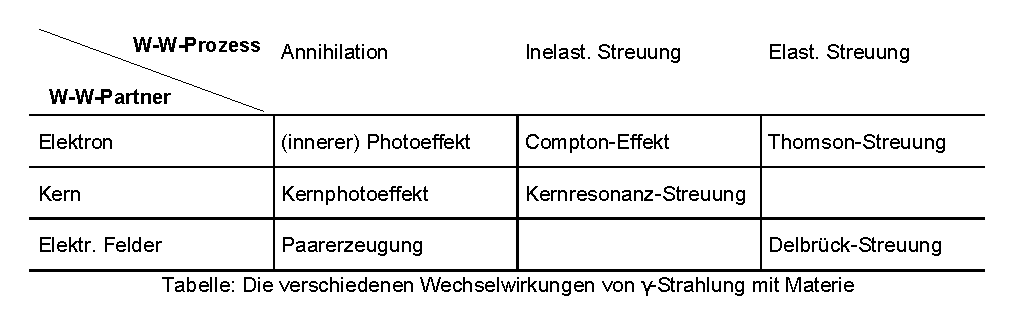
\includegraphics[width=\linewidth]{pictures/wwtabelle.pdf}
    \caption{Effekte durch Wechselwirkungen von $\gamma$-Quanten. \cite{v704}}
    \label{fig:wwtabelle}
\end{figure}

Die wichtigsten Effekte sind hierbei der Photoeffekt, der Compton-Effekt und die Paarbildung. 
Bei dem Photoeffekt wechselwirkt das $\gamma$-Quant mit einem Hüllenelektron. 
Das Elektron wird aus seiner Schale gelöst wenn die Energie des $\gamma$-Quants größer ist als die Bindungsenergie des Elektrons. 
Die übrigbleibende Energie des Photons wird dann an des Elektron abgegeben wodurch das $\gamma$-Quant vernichtet wird. 
Bei dem Compton-Effekt stößt das $\gamma$-Quant lediglich ein Elektron an und gibt einen Teil seiner Energie ab. 
Durch den Stoß verändert sich die Bahn beider Teilchen, wodurch die Intensität eines $\gamma$-Strahls abnimmt. 
Der Wirkungsquerschnitt der Compton-Streuung ist definiert durch
\begin{equation} \label{eq:Compton}
    \sigma_{\text{com}} = 
    2 \pi r_{e}^{2} 
    \left(
        \frac{1+\varepsilon}{\varepsilon^{2}} 
        \left[
              \frac{2(1+\varepsilon)}{1+2 \varepsilon}-\frac{1}{\varepsilon} \ln (1+2 \varepsilon) 
        \right] 
        +\frac{1}{2 \varepsilon} \ln (1+2 \varepsilon)-\frac{1+3 \varepsilon}{(1+2 \varepsilon)^{2}}
    \right) \, .
\end{equation}
Dabei ist das Verhältnis der Quantenenergie $E_\gamma$ zur Ruheenergie des Elektrons 
\begin{align*}
    \varepsilon &= \frac{E_\gamma}{(m_0 c^2)} 
\end{align*}
und der klassische Elektroradius
\begin{align*}
    r_{e} = \frac{e_{0}^{2}}{4 \pi \varepsilon_{0} m_{0} c^{2}} &= 2,82 \cdot 10^{-15} \mathrm{~m} \, .
\end{align*}

Für den Absorptionskoeffizienten folgt damit
\begin{equation}
    \mu_\text{com}=\frac{2 N_{A} \rho}{M} \sigma_\text{com} \, .
\end{equation}
Die Paarbildung tritt auf, wenn die Quantenenergie größer als die doppelte Ruhemasse des Elektrons ist
und das $\gamma$-Quant wird unter der Bildung eines Elektrons und eines Positrons annihiliert.

Alle drei genannten Effekte treten bei dem Durchgang eines $\gamma$-Strahls durch eine Materieschicht auf
und beeinflussen daher die Bildung des Absorptionskoeffizient.
Der Photo-Effekt ist dabei im niedrigen Energiebereich definiert, während bei hohen Energien die Paarbildung ausschlaggebend ist. 
Der Compton-Effekt sorgt für eine Angleichung im mittleren Energiebereich. 
In \autoref{fig:germanium} ist ein Verlauf des Absorptionskoeffizienten $\mu$ in Abhängigkeit der Energie dargestellt.
\begin{figure}
    \centering
    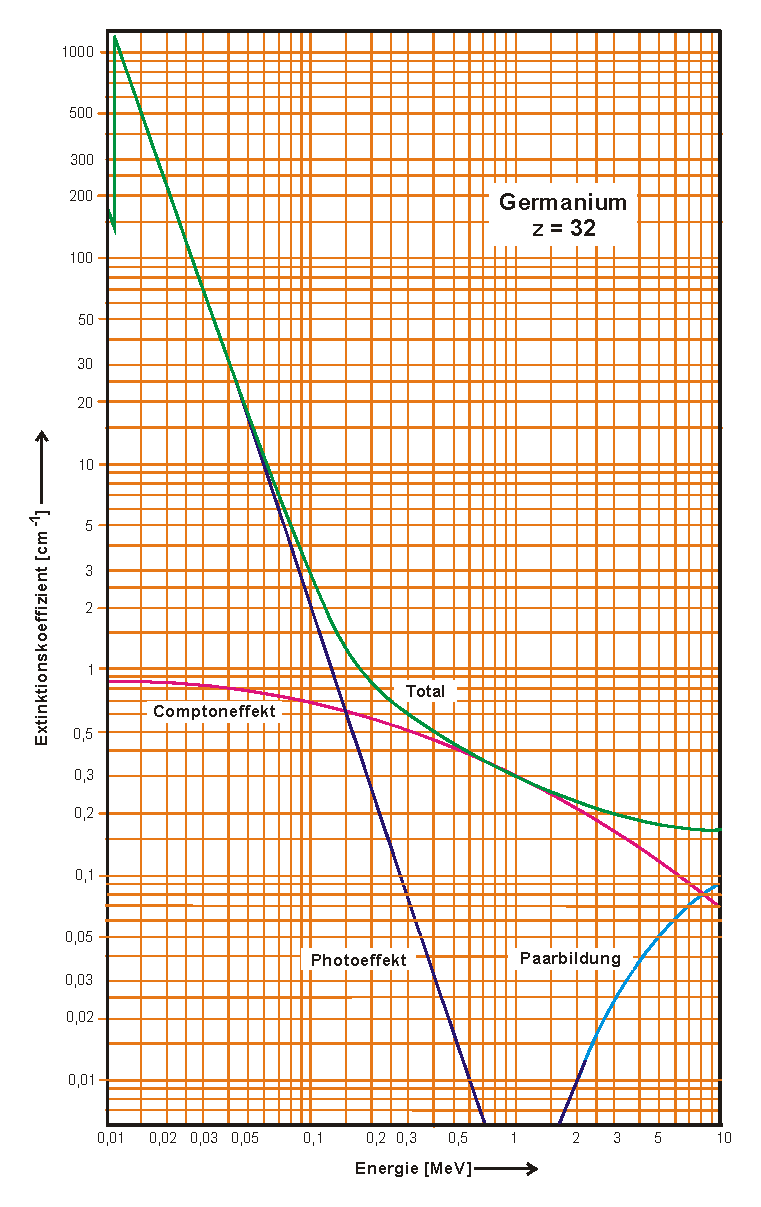
\includegraphics[width=0.6\linewidth]{pictures/germanium.pdf}
    \caption{Absorptionskoeffizient von Germanium in Abhängigkeit von der Energie. \cite{v704}}
    \label{fig:germanium}
\end{figure}


\subsection[Beta-Strahlung]{$\beta$-Strahlung}

Die $\beta$-Strahlung entsteht bei dem Zerfall von Atomkernen und besteht aus Elektronen mit hoher Geschwindigkeit:
\begin{equation}
    \mathrm{n} \rightarrow \mathrm{p}+\beta^{-}+\bar{v}_{e^{-}} \, .
\end{equation}
Bei dem $\beta^-$-Zerfall zerfällt ein Neutron in ein Proton, ein Elektron und ein Antineutrino.
Der $\beta^+$-Zerfall beschreibt wie ein Proton in ein Neutron, ein Positron und ein Neutrino zerfällt. 
Die Energie verteilt sich dabei kontinuierlich auf das Elektron/Positron und das Neutrino/Antineutrino. 
Die $\beta$-Teilchen erleiden beim Durchgang durch Materie wesentlich mehr Wechselwirkungen als bei der $\gamma$-Strahlung. 

Es werden im wesentlichen 3 Prozessen voneinander unterschieden. 
Bei der elastischen Streuung werden die $\beta$-Teilchen von dem Coulomb-Feld der Atomkerne abgelenkt, 
wodurch die $\beta$-Teilchen eine starke Ablenkung und auch geringe Energieverluste erfahren.

Bei der inelastischen Streuung werden die $\beta$-Teilchen von dem Coulomb-Feld der Atomkerne beschleunigt. 
Dadurch senden sie Energie in Form von elektromagnetischer Strahlung ab, wodurch sie abgebremst werden. 

Durch inelastische Streuung an den Elektronen des Absorbermaterials verlieren die $\beta$-Teilchen nur einen Bruchteil ihrer Energie. 
Da diese Stöße jedoch sehr häufig Auftreten können und diese Wahrscheinlichkeit proportional zur Zahl der Elektronen pro Volumeneinheit ist, 
können $\beta$-Teilchen durch diesen Prozess ihre gesamte Energie verlieren.

Aus natürlichen Quellen gilt für $\beta$-Teilchen aus natürlichen Quellen 
bei nicht allzu großen Absorberschichtdicken näherungsweise \autoref{eq:absorptionsgesetz}. 
Für Schichtdicken in der Nähe der maximalen Massenbelegung $R_\text{max}$ der Teilchen weicht das Gesetzt deutlich ab. 
Oberhalb von dieser Reichweite wird nur noch die Bremsstrahlung der $\beta$-Strahlung gemessen.
Die in \autoref{fig:massenbelegung} dargestellte Massenbelegung hängt von der Schichtdicke ab:
\begin{equation}
    R = \rho D
\end{equation}
\begin{figure}
    \centering
    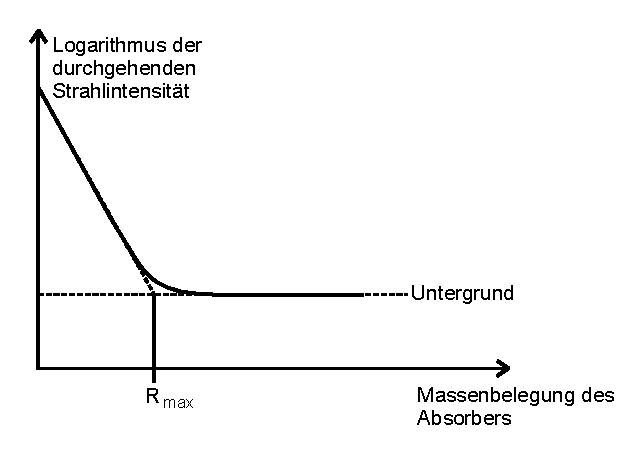
\includegraphics[width=0.6\linewidth]{pictures/massenbelegung.pdf}
    \caption{Absorptionskurve eines natürlichen $\beta$-Strahlers. \cite{v704}}
    \label{fig:massenbelegung}
\end{figure}
Da $R_\text{max}$ fast ausschließlich durch die energiereichsten Elektronen bestimmt ist, kann
daraus die Größe $E_\text{max}$ berechnet werden. 
Dies erfolgt durch die experimentell bestimmte Formel
\begin{equation} \label{eq:Emax}
    E_\text{max}= 1,92 \sqrt{R_\text{max}^{2}+ 0,22 R_\text{max}} \, .
\end{equation}